\section{Preventivo}
	In questa sezione verranno riportati i preventivi per le varie fasi di lavoro. Per facilitare la comprensione delle tabelle i ruoli verranno abbreviati con le seguenti sigle identificative:
			\begin{itemize}
			\item\textbf{Re:} Responsabile;
			\item\textbf{Am:} Amministratore;
			\item\textbf{An:} Analista;
			\item\textbf{Pg:} Progettista;
			\item\textbf{Pr:} Programmatore;
			\item\textbf{Ve:} Verificatore;
		\end{itemize}
	\subsection{Fase di Analisi}
		\subsubsection{Prospetto orario}
			Durante la fase di Analisi la distribuzione oraria preventivata dei ruoli di ogni componente del gruppo sarà la seguente:
			
			\rowcolors{2}{lightest-grayest}{white}
			\begin{longtable}{|c|c|c|c|c|c|c|c}
				\hline
				\rowcolor{lighter-grayer}
				\textbf{Nome} & \textbf{Re} & \textbf{Am} & \textbf{An} & \textbf{Pg}  & \textbf{Pr}   & \textbf{Ve} & \textbf{Totale} \\
				\hline
				\endfirsthead
				
				\hline
				Giuseppe Vito Bitetti & 0 & 9 & 9 & 0 & 0 & 12 & 30\\
				\hline
				\hline
				Lorenzo Dei Negri & 8 & 0 & 13 & 0 & 0 & 9 & 30\\
				\hline
				\hline
				Nicolò Frison & 0 & 10 & 8 & 0 & 0 & 12 & 30\\
				\hline
				\hline
				Fouad Mouad & 0 & 7 & 11 & 0 & 0 & 12 & 30\\
				\hline
				\hline
				Mariano Sciacco & 8 & 0 & 12 & 0 & 0 & 10 & 30\\
				\hline
				\hline
				Alessandro Tommasin & 11 & 0 & 10 & 0 & 0 & 9 & 30\\
				\hline
				\hline
				Giovanni Vidotto & 0 & 7 & 8 & 0 & 0 & 15 & 30\\
				\hline 

			\end{longtable}
			\pagebreak
		
			La tabella può essere riassunta nel seguente istogramma:
		
			\begin{figure}[H]
				\centering
				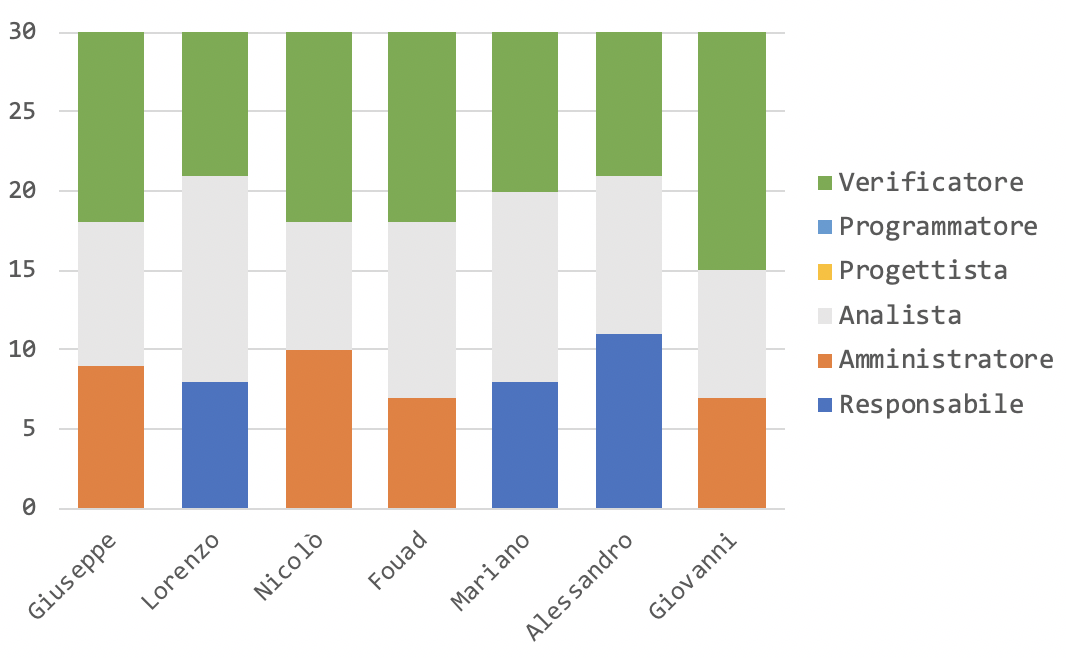
\includegraphics[width=0.8\linewidth]{./images/analisi1.png}
				\caption{Grafico ore/ruolo componenti nella fase di Analisi}
				\label{fig:grafico suddivione ruoli fase Analisi}
			\end{figure}
		
			\subsubsection{Prospetto Economico}
			In base al prospetto orario, quello economico sarà il seguente: 
			
			\rowcolors{2}{lightest-grayest}{white}
			\begin{longtable}{|c|c|c|c|c|c|c|c}
				\hline
				\rowcolor{lighter-grayer}
				\textbf{Ruolo} & \textbf{Ore} & \textbf{Costo} \\
				\hline
				\endfirsthead
				
				\hline
				Responsabile & 27 & 810\\
				\hline
				\hline
				Amministratore & 33 & 660\\
				\hline
				\hline
				Analista & 71 & 1775\\
				\hline
				\hline
				Progettista & 0 & 0\\
				\hline
				\hline
				Programmatore & 0 & 0\\
				\hline
				\hline
				Verificatore & 79 & 1185\\
				\hline
				\textbf{Totale} & 210 & 4430\\
				\hline
			
			\end{longtable}
			\pagebreak
		
			La tabella può essere riassunta nel seguente areogramma:
			\begin{figure}[H]
				\centering
				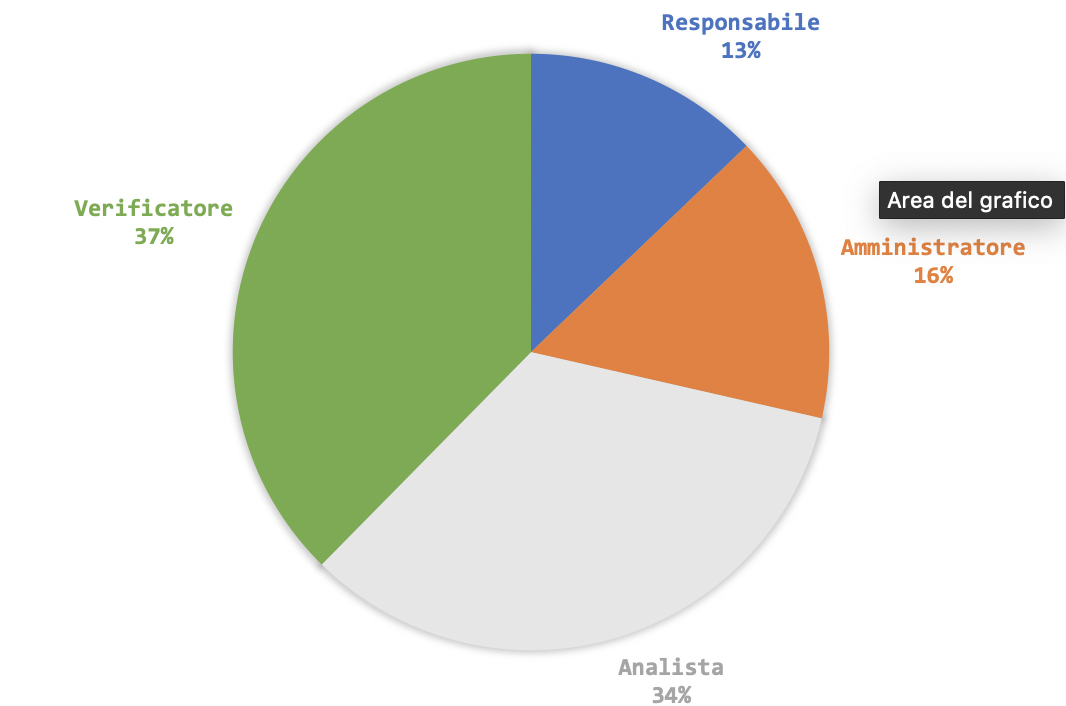
\includegraphics[width=0.8\linewidth]{./images/analisi2.png}
				\caption{Grafico percentuale ore/ruolo nella fase di Analisi dei requisiti}
				\label{fig:grafico costi ruolo fase Analisi}
			\end{figure}
		
	\subsection{Fase di Consolidamento dei requisiti}
			\subsubsection{Prospetto orario}
			Durante la fase di Consolidamento dei requisiti la distribuzione oraria preventivata dei ruoli di ogni componente del gruppo sarà la seguente:
			
			\rowcolors{2}{lightest-grayest}{white}
			\begin{longtable}{|c|c|c|c|c|c|c|c}
				\hline
				\rowcolor{lighter-grayer}
				\textbf{Nome} & \textbf{Re} & \textbf{Am} & \textbf{An} & \textbf{Pg}  & \textbf{Pr}   & \textbf{Ve} & \textbf{Totale} \\
				\hline
				\endfirsthead
				
				\hline
				Giuseppe Vito Bitetti & 0 & 0 & 5 & 0 & 0 & 0 & 5\\
				\hline
				\hline
				Lorenzo Dei Negri & 0 & 5 & 0 & 0 & 0 & 0 & 5\\
				\hline
				\hline
				Nicolò Frison & 0 & 0 & 0 & 0 & 0 & 5 & 5\\
				\hline
				\hline
				Fouad Mouad & 2 & 0 & 0 & 0 & 0 & 3 & 5\\
				\hline
				\hline
				Mariano Sciacco & 0 & 0 & 3 & 0 & 0 & 2 & 5\\
				\hline
				\hline
				Alessandro Tommasin & 0 & 0 & 4 & 0 & 0 & 1 & 5\\
				\hline
				\hline
				Giovanni Vidotto & 2 & 0 & 0 & 0 & 0 & 3 & 5\\
				\hline 
				\textbf{Totale} & 4 &  5 & 12 & 0 & 0 & 14 & 35\\
				\hline
			\end{longtable}
			\pagebreak
		
			La tabella può essere riassunta nel seguente areogramma:
			\begin{figure}[H]
				\centering
				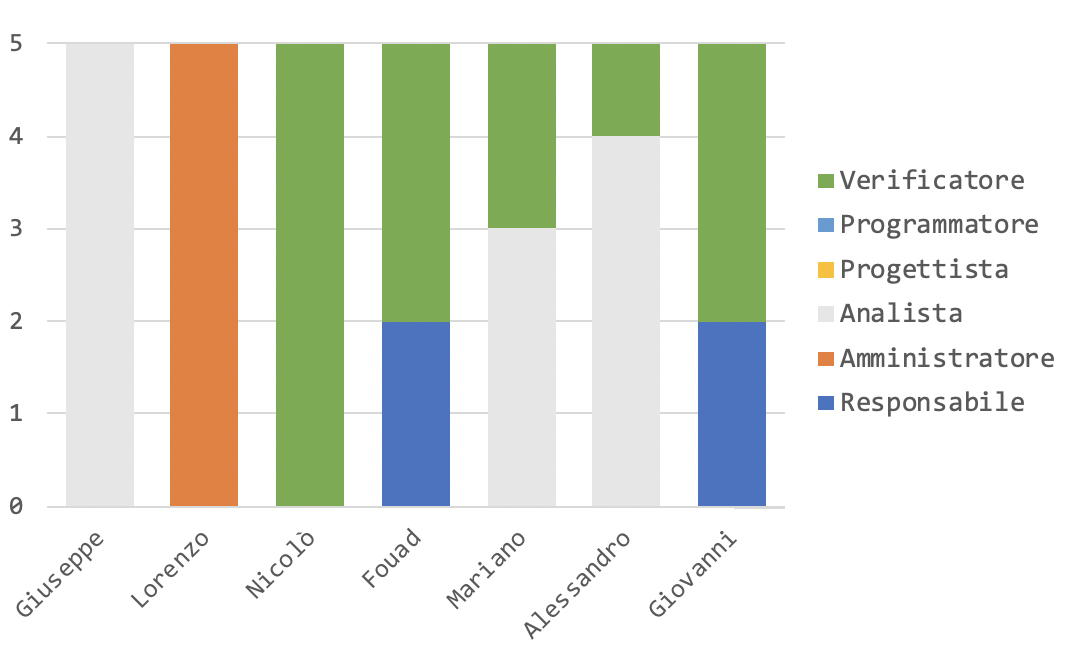
\includegraphics[width=0.8\linewidth]{./images/consRequisiti1.png}
				\caption{Grafico ore/ruolo componenti nella fase di Consolidamento dei requisiti}
				\label{fig:grafico suddivione ruoli fase Consolidamento requisiti}
			\end{figure}
		
		\subsubsection{Prospetto Economico}
		In base al prospetto orario, quello economico sarà il seguente: 
		
			\rowcolors{2}{lightest-grayest}{white}
			\begin{longtable}{|c|c|c|c|c|c|c|c}
				\hline
				\rowcolor{lighter-grayer}
				\textbf{Ruolo} & \textbf{Ore} & \textbf{Costo} \\
				\hline
				\endfirsthead
				
				\hline
				Responsabile & 4 & 120\\
				\hline
				\hline
				Amministratore & 5 & 100\\
				\hline
				\hline
				Analista & 12 & 300\\
				\hline
				\hline
				Progettista & 0 & 0\\
				\hline
				\hline
				Programmatore & 0 & 0\\
				\hline
				\hline
				Verificatore & 14 & 210\\
				\hline
				\textbf{Totale} & 35 & 730\\
				\hline
				
			\end{longtable}
			\pagebreak
			
			La tabella può essere riassunta nel seguente areogramma:
			\begin{figure}[H]
				\centering
				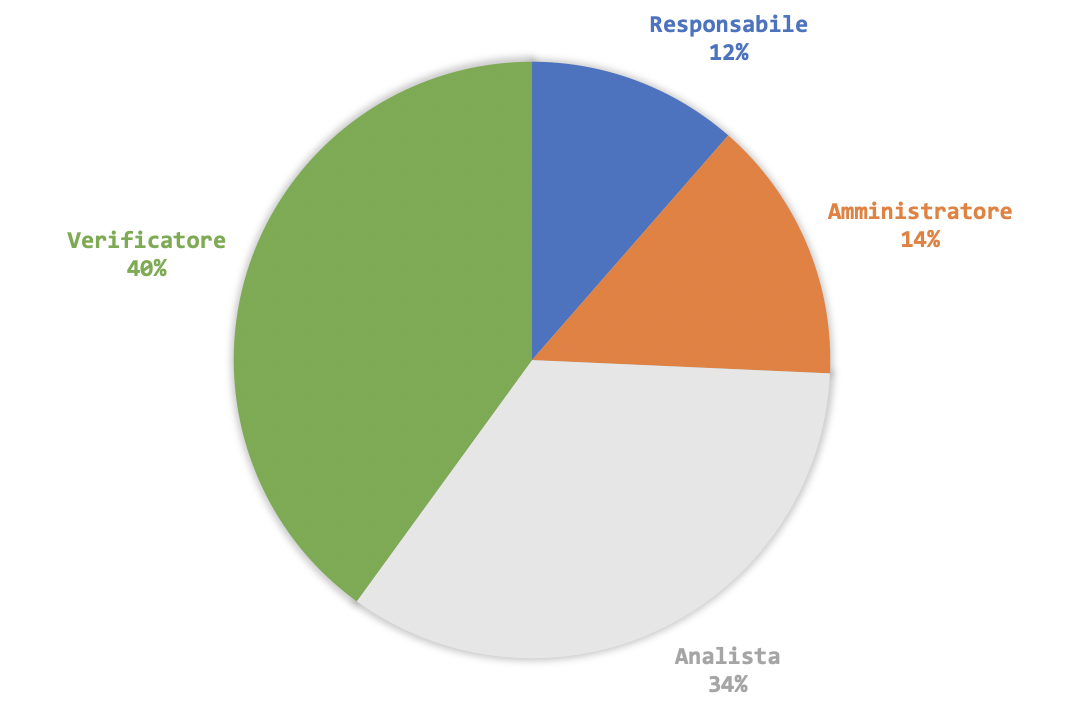
\includegraphics[width=0.8\linewidth]{./images/consRequisiti2.png}
				\caption{Grafico percentuale ore/ruolo nella fase di Consolidamento dei requisiti}
				\label{fig:grafico costi ruolo fase Consolidamento dei requisiti}
			\end{figure}
	
	\subsection{Fase di Progettazione dell'architettura}
		\subsubsection{Prospetto orario}
		Durante la fase di Progettazione la distribuzione oraria preventivata dei ruoli di ogni componente del gruppo sarà la seguente: